
In this chapter, we will mainly discuss about the \textbf{Ruby Laser} which is a solid-state laser and was the very first laser ever built (in 1960) by Theodore Maiman. Although modern lasers have evolved and use different constructions for the lasing process, they follow the same fundamental principles for the laser operation as in \textbf{Ruby Laser}.

\subsubsection{Ruby Laser}

Ruby is a crystalline solid composed of Aluminium Oxide $(Al_2O_3)$ with some traces of Chromium $(Cr^{3+})$ replacing few $Al^{3+}$ ions in the crystal lattice. These $Cr^{3+}$ ions are the reason why Ruby glows red. \vspace{.2cm}

Naturally occurring Ruby will have lot of impurities which makes it not a very good medium for concentrated laser beam to travel (will get dispersed by impurities). So for the sake of lasers, artifically made ruby crystals (i.e. $Al_2O_3$ crystals dopes with $Cr^{3+}$ ions) are used. \vspace{.2cm}

\begin{figure}[H]
    \centering
    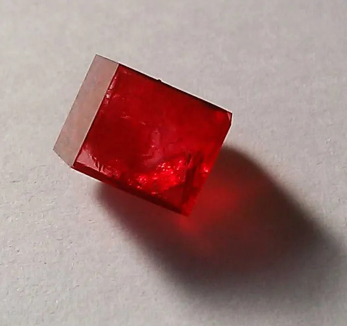
\includegraphics[scale=.8]{./img/11_ruby_crystal.png}
    \caption{Synthetic Ruby crystal}
\end{figure}

In the beginning of the chapter, we discussed about how energy levels in the solids come very close and form energy bands. But, in the case of ruby crystal, $Al_2O_3$ does form energy bands but the traces of $Cr^{3+}$ has discrete energy levels. \vspace{.2cm}

\uline{Why does $Cr^{3+}$ have discrete energy levels despite being solid?} The $Cr^{3+}$ ions have different energy levels and orbitals to interact with the energy levels and orbitals of $Al^{3+}$ ions in the crystal and form energy bands. Also, the $Cr^{3+}$ ions are present in trace amounts so they are far from each other to interact with each other and form energy bands (like in the Band theory of Solids). \vspace{.2cm}

In the whole Ruby crystal, we are only interested with the $Cr^{3+}$ ions. Infact, it is the $Cr^{3+}$ ions in the Ruby crystal which will be taking part in the stimulated emission for the lasing process. \uline{Why?} This will be explained later but it has do with how $Cr^{3+}$ ions are responsible for making Ruby glow red.